\documentclass[a4paper,11pt]{article}
\usepackage[T1]{fontenc}
\usepackage[utf8]{inputenc}
\usepackage{lmodern}
\usepackage{tikz}
\title{Navier Stokes}
\author{Ataias Reis}

\begin{document}

\section{Navier Stokes}
Quer-se resolver a seguinte equação:

\begin{eqnarray}
\rho\left( \frac{\partial \textbf{v}}{\partial
t}+\textbf{v}\cdot\nabla\textbf{v}\right)=-\nabla
p+\mu\nabla^2\textbf{v}+\textbf{f}\\
 \nabla\cdot \textbf{v}=0
\end{eqnarray}
\subsection{Resolução Numérica}
\subsubsection{Desconsiderando a pressão}
\paragraph{} Desconsiderando $\nabla p$ por agora, e notando que a parte da diferente é avaliada no tempo atual, não no futuro, tem-se:

\begin{eqnarray}
\textbf{v}_{ij}^s=(u_{i+1j}+u_{i-1j}+u_{ij+1}+u_{ij-1},v_{i+1j}+v_{i-1j}+v_{ij+1}+v_{ij-1})\\
\textbf{v}_{ij}^t=\frac{1}{4}(u_{ij}+u_{i+1j}+u_{i+1j-1}+u_{ij-1},v_{ij}+v_{i-1j}+v_{i-1j+1}+v_{ij+1})
\end{eqnarray}
\begin{eqnarray}
u_{ij}^{*}&=&\left[\frac{\mu}{\rho}\left(\frac{u_{ij}^s-4u_{ij}}{\Delta
x^2}\right)+\frac{1}{\rho}\frac{f_{x,ij}+f_{x,i-1j}}{2}\right] + u_{ij}\nonumber \\
&-&\left[u_{ij}\frac{u_{i+1j}-u_{i-1j}}{2\Delta
x}-v_{ij}^t\frac{u_{ij+1}-u_{ij-1}}{2\Delta x}\right]\Delta t
\end{eqnarray}

\begin{eqnarray}
v_{ij}^{*}&=&\left[\frac{\mu}{\rho}\left(\frac{v_{ij}^s-4v_{ij}}{\Delta
x^2}\right)+\frac{1}{\rho}\frac{f_{y,ij}+f_{y,ij-1}}{2}\right] + v_{ij}\nonumber \\
&-&\left[u_{ij}^t\frac{v_{i+1j}-v_{i-1j}}{2\Delta
x}-v_{ij}\frac{v_{ij+1}-v_{ij-1}}{2\Delta x}\right]\Delta t
\end{eqnarray}

\paragraph{} Com isto, tem-se \[\textbf{v}^{*}=(u^*,v^*)\]
\subsubsection{Obter a pressão}
\paragraph{} Tirando o divergente das equações vetoriais, tem-se a seguinte equação:
\begin{equation}
\nabla^2 p = \frac{\rho}{\Delta t} \nabla\cdot \textbf{v}^*=\frac{\rho}{\Delta t} 
\left( \frac{\partial u^*}{\partial x}+\frac{\partial v^*}{\partial y} \right)
\end{equation}
\paragraph{} Dado ter-se um sistema resolvendo a equação de poisson, basta-se calcular o termo da direita e colocar como não-homogeneidade.
\begin{equation}
DIV_{ij}=\frac{\rho}{\Delta t}\left( \frac{u_{i+1j}^*-u_{ij}^*}{\Delta x}+\frac{v_{ij+1}^*-v_{ij}^*}{\Delta x}\right)
\end{equation}
\paragraph{} As condições de contorno são todas de Neumann. Para pontos internos à malha, tem-se:
\begin{equation}
p_{ij}=\frac{1}{4}[(p_{i+1j}+p_{i-1j}+p_{ij+1}+p_{ij-1})-\Delta x^2 DIV_{ij}]
\end{equation}
\paragraph{} Quais pontos são internos à malha? São os pontos $x_{ij}$ em $D$ que é definido da seguinte maneira:
\begin{equation}
D = \{x_{ij}\,|\, 0\le i < N \textrm{ e } 0\le j < N \}
\end{equation}
\paragraph{} A rotina para Poisson com Neumann já está implementada. Falta agora
as condições de contorno nas fronteiras. Como obtê-las?
\paragraph{} Primeiramente, considere-se novamente a equação de Navier Stokes:
\[\rho\left( \frac{\partial \textbf{v}}{\partial t}+\textbf{v}\cdot\nabla\textbf{v}\right)=-\nabla p+\mu\nabla^2\textbf{v}+\textbf{f}\]
\[\nabla\cdot\textbf{v}=0\]
\paragraph{} Destrinchando a equação para duas coordenadas, tem-se:
\begin{eqnarray}
\frac{\partial u}{\partial t}+u\frac{\partial u}{\partial x}+v\frac{\partial
u}{\partial y}=-\frac{1}{\rho}\frac{\partial p}{\partial
x}+\nu\left(\frac{\partial^2 u}{\partial^2 x}+\frac{\partial^2 u}{\partial^2
y}\right)+f_x\\
\frac{\partial v}{\partial t}+u\frac{\partial v}{\partial x}+v\frac{\partial
v}{\partial y}=-\frac{1}{\rho}\frac{\partial p}{\partial
y}+\nu\left(\frac{\partial^2 v}{\partial^2 x}+\frac{\partial^2 v}{\partial^2
y}\right)+f_y
\end{eqnarray}
\paragraph{} Se fizermos uma análise dos pontos na parede da esquerda ou
direita, e aplicarmos as condições de impenetrabilidade e não-deslizamento, que
dizem que $u=0$ e $v=0$ na parede, temos a simplificação da equação, pois vários
termos se tornam zero. As equações para as duas paredes verticais é a seguinte:
\begin{equation}
\frac{\partial p}{\partial x}\Bigg|_{\textrm{parede}}=\rho\nu\frac{\partial^2
u}{\partial x^2}\Bigg|_{\textrm{parede}}+\rho f_x
\end{equation}
\paragraph{} Para as paredes que ficam na horizontal tem-se:
\begin{equation}
\frac{\partial p}{\partial y}\Bigg|_{\textrm{parede}}=\rho\nu\frac{\partial^2
v}{\partial y^2}\Bigg|_{\textrm{parede}}+\rho f_y
\end{equation}
\paragraph{Equações discretizadas para fronteira de Poisson} As equações, em
sequência, para as fronteiras da esquerda, direita, baixo e topo da matriz são
as seguintes:
\begin{eqnarray}
\frac{p_{0j}-p_{-1j}}{\Delta x}=\frac{\rho\nu}{\Delta x^2}(2u_{ij}-5u_{i+1j}+4u_{i+2j}-u_{i+3j})+\frac{\rho}{2}(f_{ij}+f_{i+1j})\\
\frac{p_{nj}-p_{n-1j}}{\Delta x}=\frac{\rho\nu}{\Delta x^2}(2u_{ij}-5u_{i-1j}+4u_{i-2j}-u_{i-3j})+\frac{\rho}{2}(f_{ij}+f_{i-1j})\\
\frac{p_{i0}-p_{i-1}}{\Delta y}=\frac{\rho\nu}{\Delta y^2}(2v_{ij}-5v_{ij+1}+4v_{ij+2}-v_{ij+3})+\frac{\rho}{2}(f_{ij}+f_{ij-1})\\
\frac{p_{in}-p_{in-1}}{\Delta y}=\frac{\rho\nu}{\Delta y^2}(2v_{ij}-5v_{ij-1}+4v_{ij-2}-v_{ij-3})+\frac{\rho}{2}(f_{ij}+f_{ij-1})
\end{eqnarray}
\paragraph{} Agora, tem-se as equações que serão utilizadas no domínio em questão, na malha escalonada, para resolver a equação da pressão em Navier Stokes. Abaixo tem-se o nosso domínio.

\tikzstyle{help lines}+=[dashed]% aaarghhh!!!
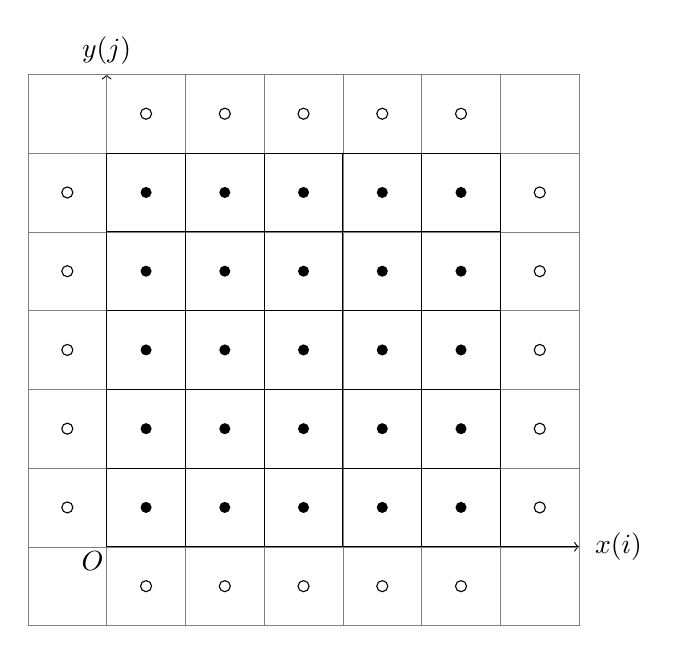
\begin{tikzpicture}
%\draw (0,0) -- (xyz cs:x=3);
%\draw (0,0) -- (xyz cs:y=3);

\draw[->] (0,5) -- (xyz cs:y=6);
\draw (0,6.3) node {$y(j)$};
\draw[->] (5,0) -- (xyz cs:x=6);
\draw (6.5,0) node {$x(i)$};
\draw (-0.18,-0.18) node {$O$};

\draw[style=help lines] (-1,-1) grid +(7,7);
\draw (0,0) grid +(5,5);
%\fill (canvas cs:x=-0.5cm,y=-0.5cm) circle (2pt);
\draw (0.5,-0.5) circle (2pt);
\draw (1.5,-0.5) circle (2pt);
\draw (2.5,-0.5) circle (2pt);
\draw (3.5,-0.5) circle (2pt);
\draw (4.5,-0.5) circle (2pt);
%\fill (canvas cs:x=5.5cm,y=-0.5cm) circle (2pt);
\draw (-0.5,0.5) circle (2pt);
\fill (canvas cs:x=0.5cm,y=0.5cm) circle (2pt);
\fill (canvas cs:x=1.5cm,y=0.5cm) circle (2pt);
\fill (canvas cs:x=2.5cm,y=0.5cm) circle (2pt);
\fill (canvas cs:x=3.5cm,y=0.5cm) circle (2pt);
\fill (canvas cs:x=4.5cm,y=0.5cm) circle (2pt);
\draw (5.5,1.5) circle (2pt);
\draw (5.5,0.5) circle (2pt);
\draw (-0.5,1.5) circle (2pt);
\fill (canvas cs:x=0.5cm,y=1.5cm) circle (2pt);
\fill (canvas cs:x=1.5cm,y=1.5cm) circle (2pt);
\fill (canvas cs:x=2.5cm,y=1.5cm) circle (2pt);
\fill (canvas cs:x=3.5cm,y=1.5cm) circle (2pt);
\fill (canvas cs:x=4.5cm,y=1.5cm) circle (2pt);
\draw (-0.5,2.5) circle (2pt);
\fill (canvas cs:x=0.5cm,y=2.5cm) circle (2pt);
\fill (canvas cs:x=1.5cm,y=2.5cm) circle (2pt);
\fill (canvas cs:x=2.5cm,y=2.5cm) circle (2pt);
\fill (canvas cs:x=3.5cm,y=2.5cm) circle (2pt);
\fill (canvas cs:x=4.5cm,y=2.5cm) circle (2pt);
\draw (5.5,2.5) circle (2pt);
\draw (-0.5,3.5) circle (2pt);
\fill (canvas cs:x=0.5cm,y=3.5cm) circle (2pt);
\fill (canvas cs:x=1.5cm,y=3.5cm) circle (2pt);
\fill (canvas cs:x=2.5cm,y=3.5cm) circle (2pt);
\fill (canvas cs:x=3.5cm,y=3.5cm) circle (2pt);
\fill (canvas cs:x=4.5cm,y=3.5cm) circle (2pt);
\draw (5.5,3.5) circle (2pt);
\draw (-0.5,4.5) circle (2pt);
\fill (canvas cs:x=0.5cm,y=4.5cm) circle (2pt);
\fill (canvas cs:x=1.5cm,y=4.5cm) circle (2pt);
\fill (canvas cs:x=2.5cm,y=4.5cm) circle (2pt);
\fill (canvas cs:x=3.5cm,y=4.5cm) circle (2pt);
\fill (canvas cs:x=4.5cm,y=4.5cm) circle (2pt);
\draw (5.5,4.5) circle (2pt);
%\fill (canvas cs:x=-0.5cm,y=5.5cm) circle (2pt);
\draw (0.5,5.5) circle (2pt);
\draw (1.5,5.5) circle (2pt);
\draw (2.5,5.5) circle (2pt);
\draw (3.5,5.5) circle (2pt);
\draw (4.5,5.5) circle (2pt);
%\fill (canvas cs:x=5.5cm,y=5.5cm) circle (2pt);
%\draw[style=help lines] (0.7,0.5) rectangle (2.3,2.5);
%\draw (0,0) rectangle (1.5,1.5);
%\draw[style=help lines] (0.5,0.7) rectangle (2.5,2.3);
\end{tikzpicture}

\paragraph{} Cada um dos pontos pretos são pontos internos, e nestes pontos precisamos saber os valores das derivadas, de forma a obter a matriz $DIV$, para então utilizar na resolução da equação de Navier, que estamos originalmente interessados. Com a malha extendida, com a fronteira imaginária adicionada, ela fica no ``ponto'' para obter o gradiente de pressão usando derivadas centrais em cada um dos pontos, agora internos, da nossa malha extendida.

\subsubsection{Resolver para o passo $t+\Delta t$}
\paragraph{} Finalmente, tem-se:
\begin{equation}
\frac{\textbf{v}^{n+1}-\textbf{v}^*}{\Delta t}=-\frac{1}{\rho}\nabla p
\end{equation}
\paragraph{} Expandindo para as equações escalares, tem-se:
\begin{eqnarray}
u^{n+1}=u^*-\frac{\Delta t}{\rho}\frac{\partial p}{\partial x}\\
v^{n+1}=v^*-\frac{\Delta t}{\rho}\frac{\partial p}{\partial y}
\end{eqnarray}
\paragraph{} Basta discretizar os termos das derivadas parciais agora:

\begin{eqnarray}
p_{x,ij}=\frac{p_{ij}-p_{i-1j}}{\Delta x}\\
p_{y,ij}=\frac{p_{ij}-p_{ij-1}}{\Delta x}
\end{eqnarray}

\paragraph{} E finalmente tem-se a solução para o tempo $n+1$ a partir do tempo passado $n$:

\begin{eqnarray}
u^{n+1}=u^*-\frac{\Delta t}{\rho}p_x\\
v^{n+1}=v^*-\frac{\Delta t}{\rho}p_y
\end{eqnarray}
\paragraph{} Cada uma das varíaveis acima é uma matriz.
\end{document}
